\chapter{\IfLanguageName{dutch}{Stand van zaken}{State of the art}}%
\label{ch:stand-van-zaken}

% Tip: Begin elk hoofdstuk met een paragraaf inleiding die beschrijft hoe
% dit hoofdstuk past binnen het geheel van de bachelorproef. Geef in het
% bijzonder aan wat de link is met het vorige en volgende hoofdstuk.

% Pas na deze inleidende paragraaf komt de eerste sectiehoofding.

%Dit hoofdstuk bevat je literatuurstudie. De inhoud gaat verder op de inleiding, maar zal het onderwerp van de bachelorproef *diepgaand* uitspitten. De bedoeling is dat de lezer na lezing van dit hoofdstuk helemaal op de hoogte is van de huidige stand van zaken (state-of-the-art) in het onderzoeksdomein. Iemand die niet vertrouwd is met het onderwerp, weet nu voldoende om de rest van het verhaal te kunnen volgen, zonder dat die er nog andere informatie moet over opzoeken \autocite{Pollefliet2011}.

%Je verwijst bij elke bewering die je doet, vakterm die je introduceert, enz.\ naar je bronnen. In \LaTeX{} kan dat met het commando \texttt{$\backslash${textcite\{\}}} of \texttt{$\backslash${autocite\{\}}}. Als argument van het commando geef je de ``sleutel'' van een ``record'' in een bibliografische databank in het Bib\LaTeX{}-formaat (een tekstbestand). Als je expliciet naar de auteur verwijst in de zin, gebruik je \texttt{$\backslash${}textcite\{\}}.
%Soms wil je de auteur niet expliciet vernoemen, dan gebruik je \texttt{$\backslash${}autocite\{\}}. In de volgende paragraaf een voorbeeld van elk.

%\textcite{Knuth1998} schreef een van de standaardwerken over sorteer- en zoekalgoritmen. Experten zijn het erover eens dat cloud computing een interessante opportuniteit vormen, zowel voor gebruikers als voor dienstverleners op vlak van informatietechnologie~\autocite{Creeger2009}.

%\lipsum[7-20]

Als eerste stap in dit onderzoek, wordt een literatuurstudie opgesteld. Hierin wordt zo veel mogelijk bestaande informatie over de onderzoeksvraag verzameld. Voor dit onderzoek zal vooral informatie vergaard worden over machine learning, de verschillende manieren om de afstand tussen strings te berekenen en de mogelijkheden om de data te clusteren op basis van die afstanden.


\section{Machine learning}
Machine learning staat centraal in dit onderzoek. Er bestaan drie belangrijke types machine learning algoritmen.

\subsection{Gesuperviseerd leren}
Als eerste is er het gesuperviseerd leren: hierbij bevat iedere waarde onmiddellijk een label met het juiste antwoord. Eenvoudig voorbeeld: als er een algoritme gesuperviseerd wordt getraind om katten te herkennen op foto's, dan bevat iedere foto die getoond wordt aan het algoritme een label met 'ja' of 'nee'. Als het algoritme dan goed genoeg getraind is, is het in staat om foto's zonder label, het juiste label te geven \autocite{Postma2019}.
\\\indent
\subsection{Ongesuperviseerd leren}
Het tweede type is ongesuperviseerd leren. Dit is logischerwijs het omgekeerde van gesuperviseerd leren. In ons simpel voorbeeld van de katten, ontvangt het algoritme een grote dataset met foto's. Dit algoritme zoekt vervolgens in deze set naar iets dat overeenkomt in veel van de foto's. Deze overeenkomst wordt in de ogen van het algoritme de 'kat'. Vervolgens splitst het de foto's in twee groepen. Eén die de 'kat' wel bevat en één die hem niet bevat. Aangezien er geen labels hangen aan de dataset, kan het algoritme zelf niet weten of het juist of fout is. Dit zorgt ervoor dat er minder controle is over de uitkomst, waardoor deze methode minder succesvol is. Zo kan het natuurlijk gebeuren dat veel foto's, naast een kat, ook een boom bevatten. Hierdoor kan het gebeuren dat het algoritme de foto's splitst in een groep met boom en zonder boom, want het algoritme kan niet weten hoe een kat eruitziet. Waarom zou ongesuperviseerd leren dan gebruikt worden als het minder succesvol is? In het voorbeeld van de katten is het inderdaad niet zo moeilijk om een label 'ja' of 'nee' aan iedere foto te geven, maar in heel veel andere gevallen kunnen er geen labels aan de data gegeven worden en kan het enorm handig zijn als het algoritme gewoon de data zonder labels in verschillende groepen verdeelt. Dit geeft al veel inzicht in de data \autocite{Postma2019}.

\subsection{Reinforcement learning}
Het derde type is reinforcement learning. Dit wordt veel gebruikt bij situaties waarin het algoritme een juiste volgorde van acties moet uitvoeren. Iedere keer dat het algoritme correct is, wordt het beloond. Deze methode wordt ook gebruikt voor het aanleren van gedrag bij dieren. Als een hond getraind wordt om te zitten bijvoorbeeld, krijgt hij een snoepje of aaitje iedere keer hij het commando goed uitvoert \autocite{Postma2019}.

\\\indent
\\\indent
In dit onderzoek wordt gebruik gemaakt van ongestructureerde masterdata, dit betekent dat de data geen labels bevat. De bedoeling is om de data te onderverdelen in gelijkaardige groepen. Het is dus vanzelfsprekend dat ongesuperviseerd leren gebruikt wordt in dit onderzoek.

\section{N-grammen}
N-grammen zijn allemaal substrings van een grotere string. Deze substrings kunnen opgesteld worden met karakters of met woorden, maar meestal gebeurt dit op basis van karakters zodanig dat iedere substring $N$ karakters bevat. Als er dus met 2-grammen wordt gewerkt bestaan alle substrings uit twee karakters, wordt er met 4-grammen gewerkt, bestaan ze uit vier karakters.
\\\indent
Bijvoorbeeld voor het woord 'Hyundai' zijn alle 2-grammen: 'Hy', 'yu', 'un', 'nd', 'da' en 'ai' en alle 4-grammen zijn: 'Hyun', 'yund', 'unda' en 'ndai'. Voor een deel van van de algoritmes die in dit onderzoek gebruikt worden, worden de waarden uit de tabel eerst in $N$-grammen gesplitst \autocite{Santos2009}.

\section{Van woorden naar getallen}
Nu er beslist is dat er gebruik gemaakt wordt van ongesuperviseerd leren, komt een volgend probleem naar boven. Onze ongestructureerde masterdata bevat woorden en karakters, maar de algoritmen kunnen dit niet groeperen. Deze verwachten de data in de vorm van getallen. Er zijn verschillende manieren om dit te doen. Een eerste manier is door de afstand tussen de woorden te berekenen. Een tweede manier is door de woorden om te zetten in betekenisvolle getallen.
\\\indent
Als eerste zullen een paar methoden besproken worden om de afstand tussen twee woorden te berekenen. Twee identieke waarden onderscheiden is natuurlijk niet zo moeilijk \autocite{Lievens2022}. Het wordt een stuk lastiger om waarden te identificeren die wel gelijkend, maar niet volledig identiek zijn. Een groot voorbeeld hiervan zijn typfouten. Het is wel belangrijk om een goed algoritme te kiezen, om zo weinig mogelijk, of in het beste geval geen, vals positieve uitkomsten te krijgen \autocite{Silva2022}. In dit onderzoek wordt enkel de Levenshtein distance gebruikt om de afstand te berekenen, maar ter verduidelijking zullen er nog een paar andere methoden besproken worden.


\subsection{Levenshtein distance}
Een eerste mogelijkheid is om gebruik te maken van de 'Levenshtein distance'. Deze metriek bepaalt de afstand tussen twee strings aan de hand van het aantal uit te voeren operaties. Deze operaties zijn: een letter toevoegen of verwijderen en een letter veranderen. Hoe meer operaties er moeten uitgevoerd worden, hoe groter de afstand tussen twee strings \autocite{Wikiversity2022}.
\\\indent
\begin{figure}[h]
    \centering
    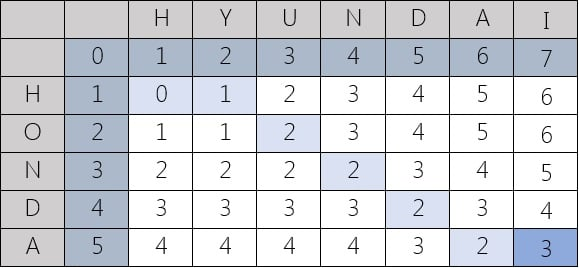
\includegraphics[width=0.7\linewidth]{../foto's/levenshtein-example}
    \caption{Een voorbeeld van de levenshtein distance waar Hyundai en Honda vergeleken worden \autocite{Cuelogic2017}.}
    \label{fig:levenshtein_voorbeeld_Hyundai_Honda}
\end{figure}
\\\indent
Een voorbeeld ter verduidelijking. De woorden 'Honda' en 'Hyundai' worden hier vergeleken. De letters van beide woorden worden op een x-as en y-as geplaatst. In de tweede rij en kolom wordt aan iedere letter een getal gegeven op basis van zijn positie in het woord. Voor Hyundai is dit dus van 0 tot en met 7 en voor Honda van 0 tot en met 5. Alle andere hokjes zijn nog niet ingevuld. Het invullen begint linksboven, eerst wordt de eerste rij volledig ingevuld van links naar rechts, dan pas wordt de volgende rij begonnen.
\\\indent
Ieder vakje wordt berekend op basis van drie voorgaande vakjes, namelijk de vakjes die zich links van, boven en linksboven het in te vullen vakje bevinden. Voor het eerste vakje zijn dit dus de getallen 1, 0 en 1. Met ieder getal wordt een berekening gedaan: de berekening voor de getallen erboven en er links van is eenvoudigweg plus 1. Voor het getal schuin linksboven worden de letters vergeleken: als ze gelijk zijn plus 0, als ze niet gelijk zijn plus 1.
\\\indent
Voor het eerste vakje zijn de berekeningen dus: 1+1=2, 1+1=2 en 0+0=0. Tot slot wordt het laagste van de drie uitkomsten ingevuld en wordt opgeschoven naar het volgende vakje er rechts naast. Als de rij klaar is, wordt de volgende rij gestart. Als de laatste rij klaar is staat de uitkomst in de rechteronderhoek van de tabel. Bij dit voorbeeld is de uitkomst drie, dit betekent dat er dus drie operaties moeten uitgevoerd worden om van het ene woord, naar het andere te gaan.
\\\indent
Er zijn een aantal voordelen aan het gebruik van de Levenshtein distance. De input hiervoor moet geen bepaald type zijn, dit kan van alles zijn. Als er andere tekens gebruikt worden, is dit geen probleem. Dit is handig als er gewerkt wordt met ongestructureerde masterdata, aangezien deze alle mogelijke gegevens kan bevatten. Een tweede voordeel is dat het heel goed overweg kan met typfouten, als er bijvoorbeeld 100 keer 'fiets' voorkomt in de data en een keer 'fies', dan zal de Levenshtein afstand niet veel verschillen, terwijl dit met andere algoritmes wel het geval kan zijn.
\\\indent
\begin{figure}[h]
    \centering
    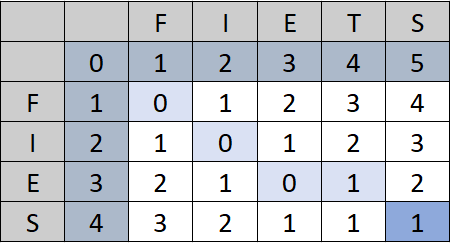
\includegraphics[width=0.7\linewidth]{../foto's/levenshteinfiets}
    \caption{Een voorbeeld van de levenshtein distance waar fiets en fies vergeleken worden.}
    \label{fig:levenshtein_voorbeeld_fiets}
\end{figure}

\subsection{Hamming distance}
Een tweede metriek om de afstand te bepalen is de 'Hamming distance'. Dit kan op twee manieren. Een eerste manier is heel gelijkaardig aan de Levenshtein distance, alleen zonder het toevoegen of verwijderen van karakters. Er wordt dus enkel gekeken hoeveel karakters verschillen. Een tweede manier transformeert eerst alle karakters in beide strings in hun binaire vorm. Bijvoorbeeld: 'a' wordt '1100001' en 'A' wordt '1000001' \autocite{Includehelp}. Vervolgens doet deze hetzelfde als de eerste manier. De afstand tussen beide strings wordt dus bepaald aan de hand van het aantal verschillen in de binaire codes van de karakters. De afstand tussen 'a' en 'A' is dus 1, aangezien er slechts één binair karakter verschilt \autocite{Silva2022}. Op onderstaande figuur is een voorbeeld te zien waar de strings 'Data A' en 'Data B' vergeleken worden.
\begin{figure}[h]
    \centering
    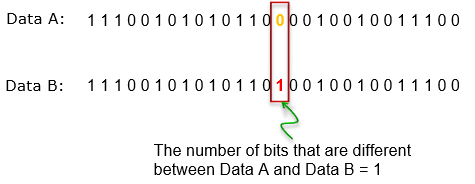
\includegraphics[width=0.7\linewidth]{../foto's/hammingdistance}
    \caption{Een voorbeeld van Hamming distance waar Data A en Data B vergeleken worden \autocite{ShareTechnote}.}
    \label{fig:hamming_distance_voorbeeld}
\end{figure}
\\\indent
Er zijn twee grote nadelen aan de hamming distance. Het eerste is het feit dat deze metriek enkel de afstand kan bepalen van strings die exact even lang zijn. In ongestructureerde masterdata is dit meestal niet het geval. Een mogelijke oplossing hiervoor is spaties toevoegen aan het einde van de kortste string zodat ze even lang worden, maar per spatie die wordt toegevoegd zal de afstand groter worden, terwijl de waarden misschien heel gelijkend zijn.
\\\indent
Een tweede nadeel van Hamming distance is het feit dat dit enkel de exact gelijke waarden eruit haalt. Als bijvoorbeeld 'fiets' en 'de fiets' worden vergeleken zullen, na drie spaties toe te voegen achter 'fiets', de letters 'f' en 'd' vergeleken worden enzovoort, waardoor deze twee strings heel ver uit elkaar zullen liggen, terwijl er in onze use case verwacht wordt dat beide waardes eigenlijk in dezelfde cluster terecht komen.

\subsection{Affine gap distance}
Een volgende metriek is de 'Affine gap distance'. Hierbij wordt er rekening gehouden met afkortingen, dit komt voornamelijk voor bij namen: 'K. Dehandschutter' in plaats van 'Kobe Dehandschutter'. Met vorige metrieken is de afstand hiertussen zeer groot, aangezien er drie letters toegevoegd moeten worden, terwijl de twee strings op zich heel gelijkaardig zijn \autocite{Walgran2019}. Qua scoring werkt het als volgt: voor elk eerste karakter dat moet aangepast worden, ook wel de opening van de gap genaamd, wordt er plus één gedaan en voor elke opvolger in de gap plus een halfje \autocite{Lievens2022}. Op onderstaande figuur is een voorbeeld te zien waarin de afstand tussen 'blvd' en 'boulevard' berekend wordt.
\\\indent
\begin{figure}[h]
    \centering
    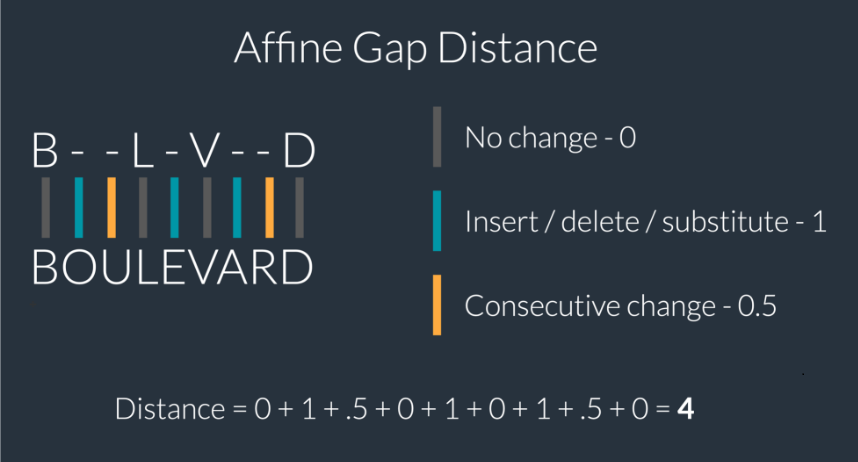
\includegraphics[width=0.7\linewidth]{../foto's/affine-gap}
    \caption{Een voorbeeld van affine gap distance waar blvd en boulevard vergeleken worden \autocite{Azavea2019}.}
    \label{fig:affine-gap}
\end{figure}


\subsection{Natural Language Processing}
Natural language processing, beter gekend als NLP, ontstond als kruispunt tussen artificiële intelligentie en taalkunde. NLP bestaat uit een grote hoeveelheid technieken die computers gebruiken om menselijke tekst te begrijpen zodat ze dit kunnen gebruiken om verschillende taken uit te voeren \autocite{Nadkarni2011}.
\\\indent
Het feit dat natuurlijke taal zo immens groot is en zo onvoorspelbaar en dubbelzinnig kan zijn, zorgde voor enkele grote problemen. Als eerste moest NLP de betekenis van de tekst kunnen achterhalen om zo de relaties tussen verschillende woorden te kunnen specificeren, denk bijvoorbeeld aan werkwoord, bijwoord, bijvoeglijk naamwoord... Daarnaast is er ook nog die dubbelzinnigheid en intonatie, als mens is het makkelijker woordmopjes of sarcasme te begrijpen, als AI is dit een enorme uitdaging \autocite{Nadkarni2011}.
\\\indent
Er zijn natuurlijk een heleboel verschillende manieren van NLP. Zo bestaat er fonologie om de klank en geluiden te herkennen van verschillende woorden. Dit wordt gebruikt om gesproken tekst te begrijpen. Ook is er morfologie, dit kijkt naar de vorm van de woorden. Hiermee kunnen prefix en suffix onderscheiden worden. In het woord 'Oneerlijk' zal bijvoorbeeld de 'on' als prefix uitkomen, wat meestal 'niet' betekent en dan blijft 'eerlijk' over, waardoor de NLP kan achterhalen dat 'oneerlijk' 'niet eerlijk' betekent. Zo zijn er nog een aantal methodes: semantisch, syntactisch, lexicaal, discourse en pragmatisch \autocite{Liddy2001}.


\subsection{Word2vec}
Bij de Levenshtein distance wordt nog geen rekening gehouden met de semantiek van de woorden. 'Frigo' en 'Koelkast' gelijken qua karakters totaal niet op elkaar, maar betekenen op zich wel hetzelfde. Om de similariteit van deze strings te berekenen, wordt elk woord omgezet in een vector via het word2vec algoritme \autocite{Lievens2022}.
\\\indent
Word2vec is op 2 verschillende manieren getraind. Als eerste is er het skip-gram algoritme.
Dit wordt gebruikt om de semantische relaties tussen woorden te modelleren door aan de hand van een woord, zijn mogelijke context te voorspellen. Als tweede is er het continuous bag-of-words (CBOW) algoritme. In tegenstelling tot het skip-gram-algoritme, gebruikt CBOW de context van een woord om het woord zelf te voorspellen. Om genoeg data te hebben om voor alle woorden een goede vector te berekenen, gebruikt word2vec het volledige wikipedia als vocabulaire \autocite{Starmer2023}.
\\\indent
Deze twee algoritmes werken zeer gelijkaardig. Alle unieke woorden uit de vocabulaire, in onderstaand voorbeeld: 'Troll2', 'is', 'great' en 'Gymkata' krijgen een inputwaarde. Deze inputs zijn verbonden met een activation function, deze neemt de som van de inputs en berekent voor iedere input een output. Aan de connecties tussen de inputs en de activation function worden gewichten gehangen, zoals te zien is op onderstaande figuur. Deze gewichten zullen bij het eindresultaat de waarde zijn die geassocieerd wordt met het woord. In het begin worden deze gewichten willekeurig gekozen. Via backpropagation zullen die gewichten aangepast worden tot ze de gewenste waarde hebben \autocite{Starmer2023}.
\begin{figure}[h]
    \centering
    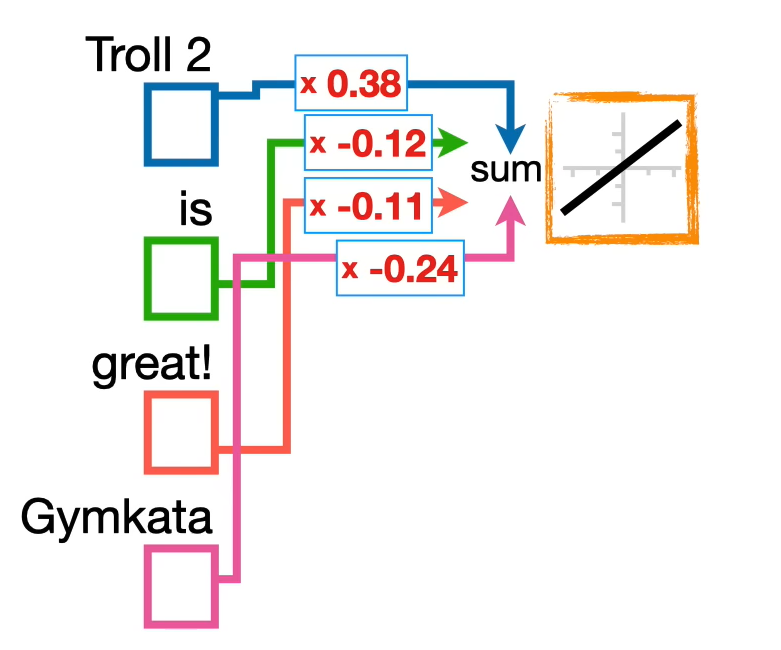
\includegraphics[width=0.7\linewidth]{../foto's/begin}
    \caption{Een grafische voorstelling van de activation functie met willekeurige gewichten \autocite{Starmer2023}.}
    \label{fig:activation_functie_met_willekeurige_gewichten}
\end{figure}

\\\indent
Backpropagation, ook wel 'achterwaartse propagatie' genoemd, is een algoritme dat wordt gebruikt voor het trainen van neurale netwerken. Backpropagation werkt door het berekenen van de afgeleiden van de verliesfunctie ten opzichte van elke gewichtsparameter in het netwerk, en vervolgens het aanpassen van deze gewichten om de fout te verminderen. De verliesfunctie wordt gebruikt om het verschil tussen de voorspelde uitkomst en de gewenste uitkomst te bepalen.
\\\indent
Het proces begint met het doorsturen van input door het netwerk om een voorspelling te genereren. Vervolgens wordt de fout tussen de voorspelde output en de werkelijke output berekend. Met behulp van de afgeleiden van de verliesfunctie worden de gewichten in het netwerk aangepast, zodat de volgende keer dat hetzelfde voorbeeld wordt doorgevoerd, de fout kleiner wordt \autocite{Starmer2023}.

\\\indent
Het skip-gram-algoritme werkt door een doelwoord te nemen en vervolgens te berekenen hoe groot de kans is dat elk ander woord uit de vocabulaire in de context van het doelwoord voorkomt \autocite{Starmer2023}.
Het skip-gram-algoritme begint met willekeurige gewichten aan ieder woord te geven, vervolgens voorspelt het aan de hand van die waarden welke woorden vaak in de context voorkomen. Het kijkt in de vocabulaire of deze voorspelling degelijk is, en past dan de gewichten aan om een beter resultaat te krijgen. Het blijft dit herhalen tot er voor ieder woord een goede waarde is waarvoor zijn context voorspeld kan worden. Het skip-gram-algoritme gebruikt ook niet één activation function, maar meestal zelfs honderd of nog meer. Aan iedere functie wordt dan een ander gewicht meegegeven per woord, en hoe meer iteraties er gebeuren, hoe dichter die gewichten bij elkaar zullen liggen. Ieder woord heeft bijgevolg een honderdtal uitkomsten en deze vectoren worden bij elkaar opgeteld. Alle opgetelde vectoren van alle woorden worden meegegeven met een softmax function. Deze functie zet de vectoren om in een getal tussen 0 en 1 zodat de som van alle getallen 1 is en hoe hoger dit getal, hoe groter de kans dat het woord in de context voorkomt, hoe kleiner dit getal, hoe kleiner de kans dat het woord in de context voorkomt \autocite{Starmer2023}.

In dit onderstaande figuur wordt er voorspeld wat de context van 'is' zou kunnen zijn, door bij 'is' als input 1 mee te geven en alle andere inputs op 0 te zetten. Op de figuur is te zien dat hier twee activation functions gebruikt worden, dus ieder woord heeft twee connecties met twee gewichten. Als eindresultaat zien we dat 'is' een waarde 0 heeft en de andere drie een waarde van 0.33, want ze hebben alledrie evenveel kans om in de context van 'is' voor te komen. Door de trainingsdata rechtsboven te bekijken, is dit een goede uitkomst \autocite{Starmer2023}.
\begin{figure}[h]
    \centering
    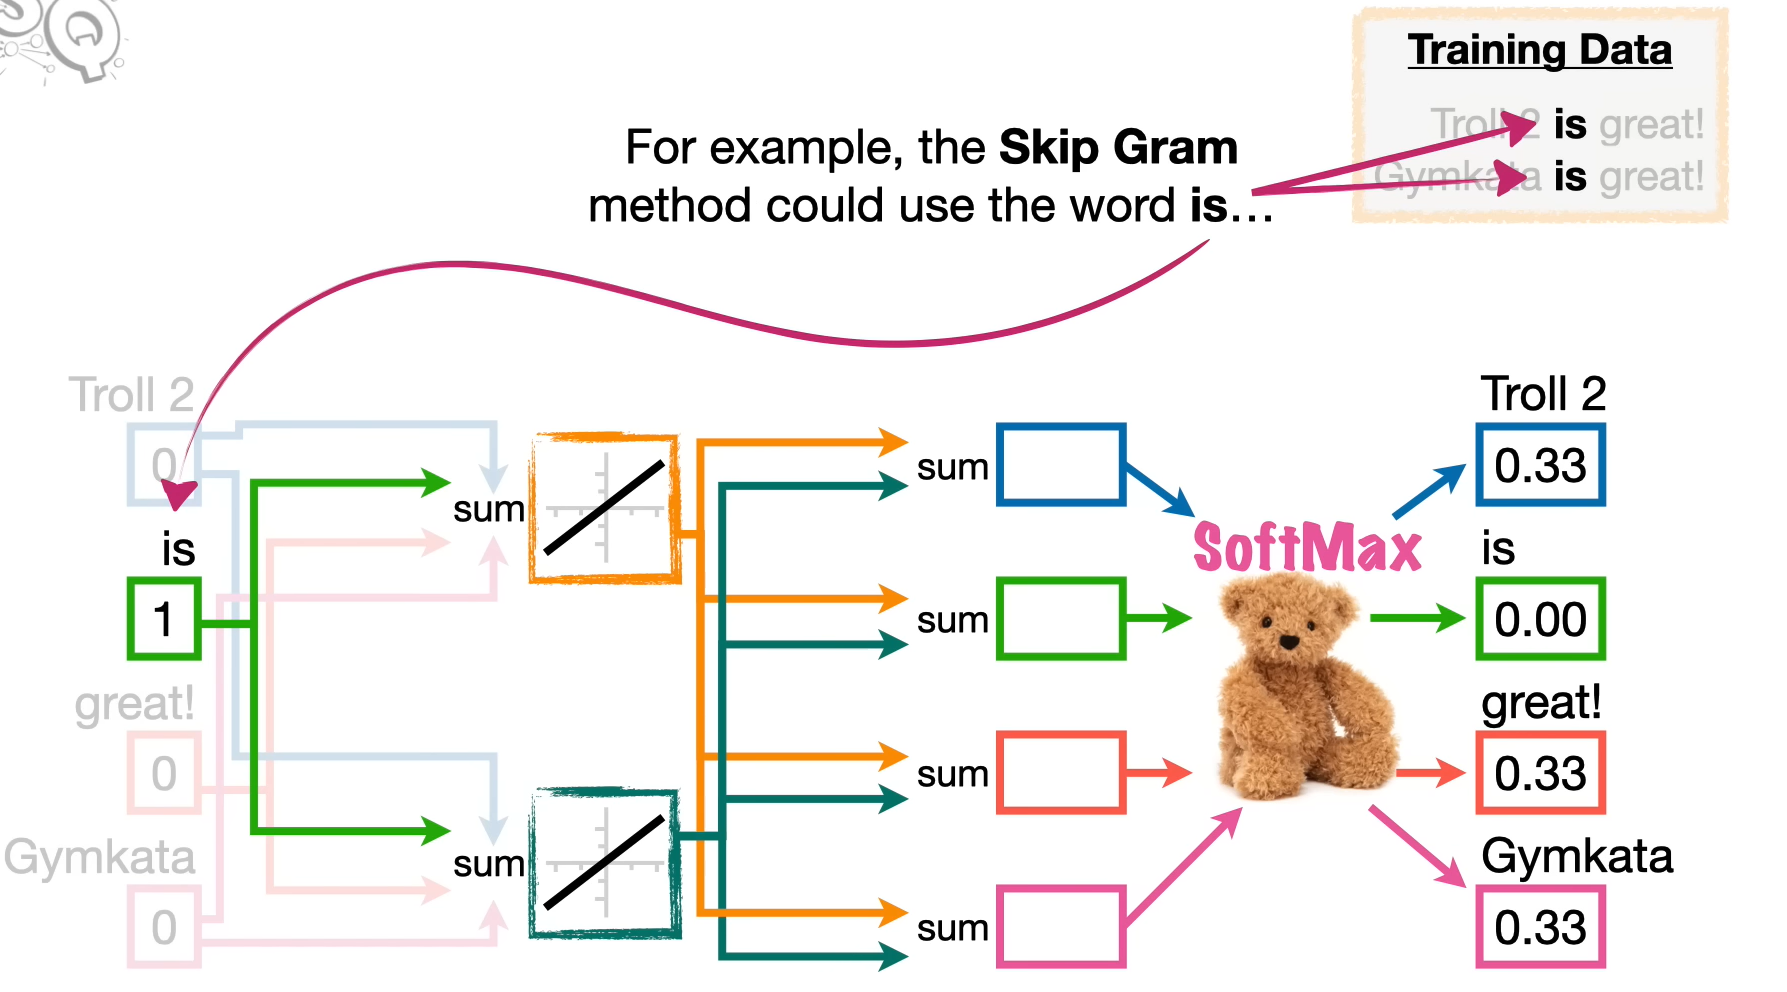
\includegraphics[width=0.7\linewidth]{../foto's/is-voorbeeld}
    \caption{Een grafische voorstelling van het eindresultaat wanneer is als input wordt gegeven \autocite{Starmer2023}.}
    \label{fig:eindresultaat_met_is_als_input}
\end{figure}
\\\indent

\\\indent
Het CBOW-algoritme werkt gelijkaardig, het neemt twee woorden en probeert vervolgens te voorspellen welk woord in het midden van deze woorden voorkomt. Meerdere woorden krijgen een 1 als input.
Het CBOW-algoritme begint ook met willekeurige waarden aan ieder woord te geven, vervolgens voorspelt het aan de hand van die waarden welke woorden in het midden kunnen staan. Het kijkt in de vocabulaire of deze voorspelling degelijk is, en past dan de gewichten aan om een beter resultaat te krijgen. Het blijft dit herhalen tot er voor iedere context een goede waarde is waarvoor het woord in het midden voorspeld kan worden. De rest van het algoritme verloopt op dezelfde manier als bij het skip-gram-algoritme \autocite{Starmer2023}.

\\\indent
Word2Vec gebruikt deze twee modellen en neemt vervolgens het gemiddelde van de twee vectoren zodat de uitkomst zo perfect mogelijk is \autocite{Starmer2023}.


\subsection{Tf-idf}
Een derde mogelijkheid is tf-idf, dit staat voor term frequency-inverse document frequency. Eerst en vooral hebben we term frequency. Dit is het aantal keer dat een woord voorkomt in het document. Dit kan berekend worden door gewoonweg te tellen hoeveel keer het voorkomt, maar als de documenten maar een paar worden bevatten, zoals in ongestructureerde masterdata toch vaak het geval is, kan dit ook berekend worden aan de hand van een boolean. Het wordt dus 1 als het document het woord bevat en 0 als het woord er niet in voorkomt. Vervolgens is er de inverse document frequency. Dit is een berekening van hoe zeldzaam het woord is ten opzichte van alle documenten in de dataset. Dit is noodzakelijk, want anders komen woorden zoals 'het', 'een', 'is' of 'er' altijd naar boven als veelgebruikte woorden. De bedoeling is dus om de woorden die niet veel voorkomen in alle documenten, maar wel regelmatig in een bepaald document voorkomen, een hoge score te geven. De idf voor een bepaald woord ($t$) in een dataset ($D$) wordt als volgt berekend: de logaritme van $N$, waarbij $N$ gelijk is aan het aantal documenten ($d$), gedeeld door het aantal documenten waarin het woord ($t$) voorkomt \autocite{Simha2021}.
\[\mathrm{idf}(t, D) = \log\bigl( \frac{N}{\mathrm{count(d \in D \colon t \in D}\bigr)})\]


Wanneer de tf en de idf berekend zijn, moeten deze nog samengevoegd worden natuurlijk. Dit wordt simpelweg gedaan door de twee waarden te vermenigvuldigen. Hoe hoger de uitkomst is, hoe belangrijker het woord is. Als de uitkomst dicht bij 0 ligt is dit woord totaal niet belangrijk \autocite{Simha2021}.


\section{Clustering}
Nu alle data uit de datasets omgezet zijn in vectoren, kan er begonnen worden met clusteren. Hiervoor worden drie verschillende methoden gebruikt. K-means, hiërarchisch en dbscan.

\subsection{K-means}
Het K-means clustering algoritme wordt gebruikt om te clusteren in een tabel met ongestructureerde data. Er moet op voorhand opgegeven worden hoeveel clusters er nodig zijn, dit is het natuurlijke getal K. Vervolgens worden er K zwaartepunten (centers) geïnitialiseerd op een random positie. Daarna wordt voor elke waarden berekend bij welk zwaartepunt ze het dichtste liggen en aan die cluster toegevoegd. Daaropvolgend start een iteratief proces waarbij voor iedere cluster het zwaartepunt wordt verlegd naar het middelpunt. Nu wordt opnieuw voor iedere waarde in de tabel berekend bij welk zwaartepunt ze het dichtst ligt en zo worden opnieuw clusters gevormd.
\\\indent
Dit iteratief proces blijft doorgaan totdat de zwaartepunten niet meer verplaatsen en de uiteindelijke clusters gevormd zijn. De dataset is dan in K clusters verdeeld. Een groot nadeel van dit algoritme is dat het getal K op voorhand moet vastliggen, terwijl het juist zeer belangrijk is dat dit getal goed gekozen wordt.
\\\indent
Een oplossing hiervoor is gebruik maken van canopy clustering. Dit is ook een clustering algoritme dat zeer snel uitgevoerd wordt, maar niet zo accuraat is. Wat wel positief is aan dit algoritme, is dat hier K niet op voorhand moet bepaald worden. Hierdoor kunnen we eerst de canopy clustering uitvoeren en aan de hand van de K die hier gebruikt wordt, het K-means algoritme uitvoeren \autocite{Vandenbussche2016}.
\\\indent
Dit algoritme heeft wel twee andere parameters nodig: T1 ofwel 'loose distance' en T2 ofwel 'tight distance' waarbij geldt dat T1 > T2. Canopy clustering begint door een willekeurige waarde te verwijderen uit de dataset en in een aparte cluster te steken, vervolgens worden alle waarden waarvan de afstand kleiner is dan T1 aan dezelfde cluster toegevoegd. Als voor deze waarden ook geldt dat de afstand kleiner is dan T2, wordt de waarde ook verwijderd uit de dataset zodat deze niet meer in andere clusters kan komen. Als de afstand tussen T1 en T2 ligt, betekent het dat de waarde wel aan de cluster wordt toegevoegd, maar dat deze ver genoeg van het centerpunt verwijderd is zodat deze waarde ook tot andere clusters kan behoren. Als deze eerste cluster klaar is, wordt opnieuw een willekeurige waarde uit de dataset verwijderd en dezelfde stappen worden uitgevoerd. Dit blijft doorgaan totdat alle waarden uit de dataset zijn verwijderd \autocite{Mahout}.

% TODO: \usepackage{graphicx} required


\subsection{Dbscan}
Dbscan is de afkorting voor Density-based spatial clustering of applications with noise. Dit is een clustering algoritme dat ontstaan is om nested clusters goed te kunnen berekenen. Dit zijn clusters die gedeeltelijk of zelfs helemaal omringd zijn door een andere cluster. Dit algoritme komt het dichtst in de buurt met hoe het menselijk oog clustert.
\\\indent
Dbscan gaat als volgt te werk: eerst telt het voor iedere waarde, het aantal punten die dicht in de buurt liggen. Dit wordt simpelweg gedaan door een cirkel te trekken rond het punt en vervolgens alle punten die in de cirkel liggen te tellen. De straal van de cirkel is één van de twee parameters die op voorhand moet worden meegegeven. De tweede parameter is het aantal dichte buren een punt nodig heeft om een Core Point te worden. Stel dat dit aantal vier is, dan worden alle punten die vier of meer punten in hun cirkel hebben een Core Point. Dit zijn meestal de punten die in het midden van een cluster liggen.
\\\indent
Vervolgens start het algoritme bij een willekeurig Core Point en dit wordt aan de eerste cluster toegevoegd. Daarna worden zijn buren bekeken en alle Core Points daarvan worden ook aan de cluster toegevoegd. Voor ieder toegevoegd punt, wordt deze stap uitgevoerd, tot er geen meer bij kunnen. Vervolgens worden voor ieder punt uit de cluster, zijn buren die geen Core Points zijn ook toegevoegd, maar dit zijn de laatste, hun buren worden niet meer toegevoegd aan deze cluster. Dit is de eerste cluster, nu wordt er terug gestart bij een willekeurig Core Point die nog niet tot een cluster behoort. Op het einde, als er geen Core Points meer overblijven, kan het zijn dat er nog punten zijn die niet tot een cluster behoren. Deze zijn de uitschieters \autocite{Starmer2022}.

\subsection{Hierarchisch}
Bij hierarchisch clusteren moet de data niet omgezet worden in getallen zoals bij K-Means of dbscan wel nodig was. Hierbij wordt gebruik gemaakt van de afstand tussen de strings. Als eerste stap wordt de eerste waarde vergeleken met alle andere waarden om te berekenen welke meest gelijkend is aan waarde 1. Deze stap wordt uitgevoerd bij iedere waarde in de dataset zodat voor elke waarde, de afstand tot zijn meest gelijkende waarde geweten is. Vervolgens wordt de kleinste afstand genomen en deze twee waarden vormen een eerste cluster \autocite{Starmer2017}.
\\\indent
Nu worden deze stappen opnieuw uitgevoerd, maar de cluster wordt vergeleken alsof het één waarde is. Op deze manier kan blijven doorgegaan worden totdat alle waarden in één cluster zitten \autocite{Starmer2017}.



\section{MoSCoW}
Om het meest geschikte algoritme te vinden zal gebruik gemaakt worden van de MoSCoW methode. Dit is een populaire methode om de vereiste eigenschappen te beheren en te prioriteren. MoSCoW is een acroniem en staat voor Must-have, Should-have, Could-have en Won't have \autocite{ProductPlan}.

\begin{enumerate}
    \item Must have: Eigenschappen die verplicht zijn, niet onderhandelbaar.
    \item Should have: Belangrijke eigenschappen die een grote waarde bijdragen, maar niet essentieel zijn.
    \item Could have: Dit zijn eigenschappen die wel een kleine bijdrage leveren, maar eerder bijzaak zijn.
    \item Won't have: Eigenschappen die voor deze situatie of dit onderzoek geen meerwaarde brengen.
\end{enumerate}







